\documentclass[tikz, border=3mm]{standalone}
\usepackage{tikz}
\usepackage{amsmath} % For \pi, \frac
\usetikzlibrary{arrows.meta, patterns.meta, positioning}

\begin{document}
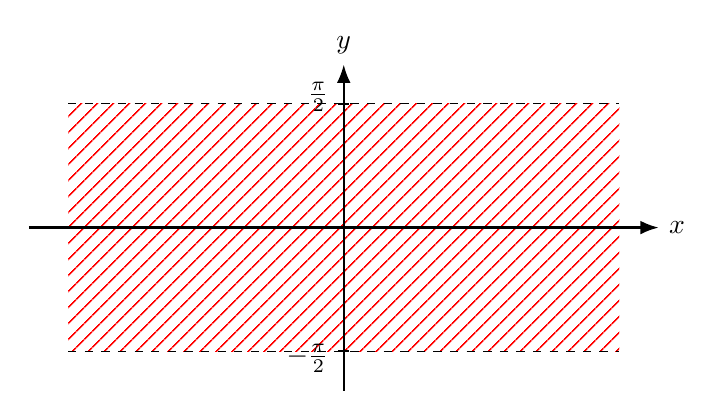
\begin{tikzpicture}[
    >=Latex, % Set default arrow tip style
    axis/.style={->, thick}, % Style for axes
    labelstyle/.style={black}, % Style for labels (black in image)
    tick/.style={thick}, % Style for tick marks
    hatchstyle/.style={pattern={Lines[angle=45, distance=4pt, line width=0.6pt]}, pattern color=red} % Hatching style
]

    % Define y-limits using pi and axis range
    \pgfmathsetmacro{\ymax}{pi/2}
    \pgfmathsetmacro{\ymin}{-pi/2}
    \def\xmax{3.5} % How far axes/lines extend horizontally
    \def\xmin{-3.5}
    \def\yaxmax{\ymax+0.5} % y-axis extends slightly beyond lines
    \def\yaxmin{\ymin-0.5}

    % --- Draw Shading First ---
    % Fill a rectangle covering the view area between ymin and ymax
    \fill[hatchstyle] (\xmin, \ymin) rectangle (\xmax, \ymax);

    % --- Draw Dashed Boundary Lines ---
    \draw[dashed] (\xmin, \ymax) -- (\xmax, \ymax);
    \draw[dashed] (\xmin, \ymin) -- (\xmax, \ymin);

    % --- Draw Axes ---
    \draw[axis] (\xmin-0.5, 0) -- (\xmax+0.5, 0) node[right] {$x$};
    \draw[axis] (0, \yaxmin) -- (0, \yaxmax) node[above] {$y$};

    % --- Ticks and Labels on y-axis ---
    % Tick and Label for pi/2
    \draw[tick] (-2pt, \ymax) -- (2pt, \ymax);
    \node[labelstyle, left=2pt] at (0, \ymax+0.09) {$\frac{\pi}{2}$};

    % Tick and Label for -pi/2
    \draw[tick] (-2pt, \ymin) -- (2pt, \ymin);
    \node[labelstyle, left=2pt] at (0, \ymin-0.09) {$-\frac{\pi}{2}$};

\end{tikzpicture}
\end{document}